In this section, we will discuss the progress of the report till now and also the work plan for the future. We will be discussing the deliverables with their timeline.

\section{Work done}
As seen earlier, the main objective of this project is to prove the non existence of functional relationship or proving that linear combination does not exist in the data records. To do so, we need to first prove that the approaches we are using is correct and true.

Hence, you can see the proofs for approaches in the previous chapter. The proofs shows that the descrepancy found in the data can help us to prove that non-functional relationship of the data. It also verifies the correctness of the approaches.

We know that the dataset provided can be small or large. Small dataset can be be verified trivially by writing an inefficient code which does all the appproaches one by one. But we know that the program must work for really large dataset as well. And larger the dataset the slower the program will become. And we would want to write an efficient algorithm.

Simple python commandline software was prototyped to create groups of the datasets by using one less performance event column. The software took input of an csv file and then grouped the data together and printed it out in a csv file with the a different name in the same directory. This was done to understand the dataset and the project.

A deep understanding of the project and research was done to understand various applications and models that have been created regarding the performance event and energy consumption.

\section{Work Plan}

Our Work plan is to first code the approaches which we have talked about. Test them with known data. Testing is an important part of the project specification.

Second main import task to make the algorithm as efficient as possible which would require creating multiple algorithms, refining and analysing them achieve maximum performance and stability as possible.

We also need to take care about the limit of data that can be processed as data can be really large to compute. Hence dividing the work into multiple small task and combining the results would be one of the options. A way to let the user enter the tolerance which could be column specific or dataset specific will be taken for the equality comparison of the values inside the column.

GUI is needed to make it easier for users to interact with the software. The GUI would allow user to take in multiple csv dataset files which would then be processed. If data descrepancy is found that proves that the dataset is not functional, would be displayed to the user in a user-friendly format. For them to know if there is a fault in the record or it might give them insight to the dataset as well.

Deliverables can now be listed:
\begin{enumerate}
    \item GUI
    \begin{enumerate}
        \item Allow users to input multiple files
        \item A way to input tolerance for multiple column
        \item Display of records that failed the test
        \item Display for the result at the end computation with simple measurements
    \end{enumerate}
    \item Core
    \begin{enumerate}
        \item Component to read csv files
        \item Multi-thread usage
        \item Finding the descrepancy in the records that fail any one of the three approaches
    \end{enumerate}
\end{enumerate}

\begin{figure}[ht]
    \centering
    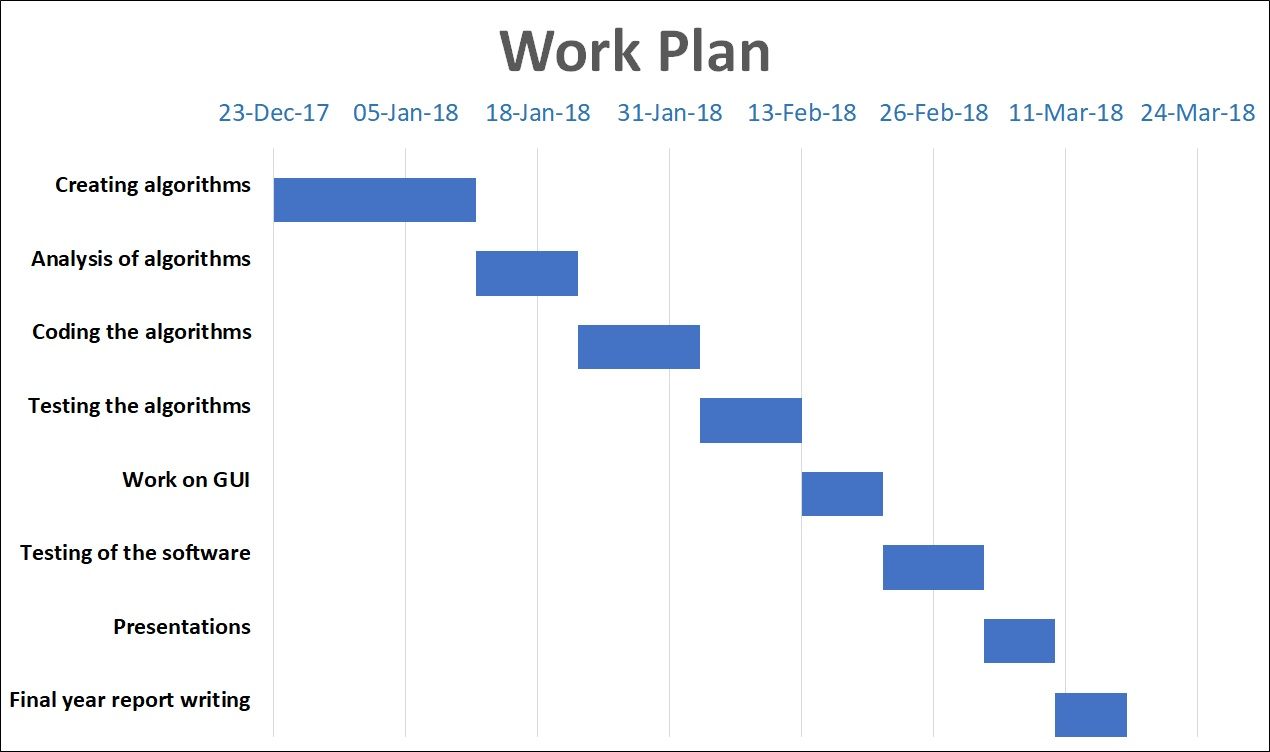
\includegraphics[width=400pt]{gantchart}
    \caption{\label{fig:gantchart} Work timeline}    
\end{figure}

As per the Fig:~\ref{fig:gantchart}, First, we will be working on the algorithm which will consist of combining all the three approaches in one and keeping track of which record broke which of the approaches rule to prove the non-existense of the function in the dataset. Second task is to anaylyse the speed of the algorithm, feasibility and stability. All the programs will then be coded into a compiled programming language. The code will be tested again several input and bugs will be fixed. GUI is the next step to give the user a friendly interface to interact with the program. Software will then be tested as a whole. Last two tasks are for completion of the presentation and final year report writing.